% **************************************************
% Document Class Definition
% **************************************************
\documentclass[%
	paper=A4,					% paper size --> A4 is default in Germany
	twoside=true,				% onesite or twoside printing
	openright,					% doublepage cleaning ends up right side
	parskip=full,				% spacing value / method for paragraphs
	chapterprefix=true,			% prefix for chapter marks
	11pt,						% font size
	headings=normal,			% size of headings
	bibliography=totoc,			% include bib in toc
	listof=totoc,				% include listof entries in toc
	titlepage=on,				% own page for each title page
	captions=tableabove,		% display table captions above the float env
	draft=false,				% value for draft version
]{scrreprt}%

% **************************************************
% Debug LaTeX Information
% **************************************************
%\listfiles

% **************************************************
% Information and Commands for Reuse
% **************************************************
\newcommand{\thesisTitle}{Seminar}
\newcommand{\thesisName}{Philipp Scholz, Anatoly Obukhov}
\newcommand{\thesisSubject}{Titel / Topic}
\newcommand{\thesisDate}{August 26, 2015}
\newcommand{\thesisVersion}{Draft / Final}

\newcommand{\thesisFirstReviewer}{Prof. Dr.-Ing. Stefan Jablonski}
\newcommand{\thesisFirstReviewerUniversity}{\protect{Universit{\"a}t Bayreuth}}
\newcommand{\thesisFirstReviewerDepartment}{Fakult{\"a}t Mathematik, Physik, Informatik}

\newcommand{\thesisSecondReviewer}{Dr. Stefan Sch{\"o}nig}
\newcommand{\thesisSecondReviewerUniversity}{\protect{Universit{\"a}t Bayreuth}}
\newcommand{\thesisSecondReviewerDepartment}{Fakult{\"a}t Mathematik, Physik, Informatik}

\newcommand{\thesisFirstSupervisor}{Stefan Sch{\"o}nig}
\newcommand{\thesisSecondSupervisor}{Lars Ackermann}

\newcommand{\thesisUniversity}{\protect{Universit{\"a}t Bayreuth}}
\newcommand{\thesisUniversityDepartment}{Fakult{\"a}t Mathematik, Physik, Informatik}
\newcommand{\thesisUniversityInstitute}{Institut f{\"u}r Informatik}
\newcommand{\thesisUniversityGroup}{Lehrstuhl f{\"u}r Angewandte Informatik IV}
\newcommand{\thesisUniversityCity}{Bayreuth}
\newcommand{\thesisUniversityStreetAddress}{Universit{\"a}tsstrasse 30}
\newcommand{\thesisUniversityPostalCode}{95447}

% **************************************************
% Load and Configure Packages
% **************************************************
\usepackage[utf8]{inputenc}		% defines file's character encoding
\usepackage[english]{babel} % babel system, adjust the language of the content
\usepackage[					% clean thesis style
	figuresep=colon,%
	sansserif=false,%
	hangfigurecaption=false,%
	hangsection=true,%
	hangsubsection=true,%
	colorize=full,%
	colortheme=bluemagenta,%
	bibsys=bibtex,%
	bibfile=bib-refs,%
	bibstyle=alphabetic,%
]{cleanthesis}

\hypersetup{					% setup the hyperref-package options
	pdftitle={\thesisTitle},	% 	- title (PDF meta)
	pdfsubject={\thesisSubject},% 	- subject (PDF meta)
	pdfauthor={\thesisName},	% 	- author (PDF meta)
	plainpages=false,			% 	-
	colorlinks=false,			% 	- colorize links?
	pdfborder={0 0 0},			% 	-
	breaklinks=true,			% 	- allow line break inside links
	bookmarksnumbered=true,		%
	bookmarksopen=true			%
}

% **************************************************
% Document CONTENT
% **************************************************
\begin{document}

% --------------------------
% rename document parts
% --------------------------
\renewcaptionname{english}{\figurename}{Fig.}
\renewcaptionname{english}{\tablename}{Tab.}

% --------------------------
% Front matter
% --------------------------
\pagenumbering{roman}			% roman page numbing (invisible for empty page style)
\pagestyle{empty}				% no header or footers
% !TEX root = ../thesis-example.tex
%
% ------------------------------------  --> cover title page
\begin{titlepage}
	\pdfbookmark[0]{Cover}{Cover}
	
\includegraphics[width=10cm]{gfx/AI4.png} \\[2mm]
		\flushright
	\vfill
	{\LARGE\thesisTitle \par}
	\rule[5pt]{\textwidth}{.4pt} \par
	{\Large\thesisName}
	\vfill
	\textit{\large\thesisDate} \\
	Version: \thesisVersion
\end{titlepage}


% ------------------------------------  --> main title page
\begin{titlepage}
	\pdfbookmark[0]{Titlepage}{Titlepage}
	\tgherosfont
	\centering

	{\Large \thesisUniversity} \\[4mm]
	\textsf{\thesisUniversityDepartment} \\
	\textsf{\thesisUniversityInstitute} \\
	\textsf{\thesisUniversityGroup} \\

	\vfill
	{\large \thesisSubject} \\[5mm]
	{\LARGE \color{ctcolortitle}\textbf{\thesisTitle} \\[10mm]}
	{\Large \thesisName} \\

	\vfill
	\begin{minipage}[t]{.27\textwidth}
		\raggedleft
		\textit{1. Reviewer}
	\end{minipage}
	\hspace*{15pt}
	\begin{minipage}[t]{.65\textwidth}
		{\Large \thesisFirstReviewer} \\
	  	{\small \thesisFirstReviewerDepartment} \\[-1mm]
		{\small \thesisFirstReviewerUniversity}
	\end{minipage} \\[5mm]
	\begin{minipage}[t]{.27\textwidth}
		\raggedleft
		\textit{2. Reviewer}
	\end{minipage}
	\hspace*{15pt}
	\begin{minipage}[t]{.65\textwidth}
		{\Large \thesisSecondReviewer} \\
	  	{\small \thesisSecondReviewerDepartment} \\[-1mm]
		{\small \thesisSecondReviewerUniversity}
	\end{minipage} \\[10mm]
	\begin{minipage}[t]{.27\textwidth}
		\raggedleft
		\textit{Supervisors}
	\end{minipage}
	\hspace*{15pt}
	\begin{minipage}[t]{.65\textwidth}
		\thesisFirstSupervisor\ 
	\end{minipage} \\[10mm]

	\thesisDate \\

\end{titlepage}


% ------------------------------------  --> lower title back for single page layout
\hfill
\vfill
{
	\small
	\textbf{\thesisName} \\
	\textit{\thesisTitle} \\
	\thesisSubject, \thesisDate \\
	Reviewers: \thesisFirstReviewer\ and \thesisSecondReviewer \\
	Supervisors: \thesisFirstSupervisor\ \\[1.5em]
	\textbf{\thesisUniversity} \\
	\textit{\thesisUniversityGroup} \\
	\thesisUniversityInstitute \\
	\thesisUniversityDepartment \\
	\thesisUniversityStreetAddress \\
	\thesisUniversityPostalCode\ \thesisUniversityCity\\ Germany
}
		% INCLUDE: all titlepages
\cleardoublepage

\pagestyle{plain}				% display just page numbers
% !TEX root = ../thesis-example.tex
%
\pdfbookmark[0]{Abstract}{Abstract}
\chapter*{Abstract}
\label{sec:abstract}
\vspace*{-10mm}

\blindtext

\vspace*{20mm}

{\usekomafont{chapter}Abstract (different language)}\label{sec:abstract-diff} \\

\blindtext
		% INCLUDE: the abstracts (english and german)
\cleardoublepage
%
\cleardoublepage
%
\setcounter{tocdepth}{2}		% define depth of toc
\tableofcontents				% display table of contents
\cleardoublepage

% --------------------------
% Body matter
% --------------------------
\pagenumbering{arabic}			% arabic page numbering
\setcounter{page}{1}			% set page counter
\pagestyle{maincontentstyle} 	% fancy header and footer

% !TEX root = ../chrysalis-report.tex
%
\chapter{Introduction}
\label{sec:intro}


In times of digitalization, \emph{Business Process Management} (BPM) systems play a central role in efficiently orchestrating and executing business processes automatically. State-of-the-art systems use a centralized program, the BPM \emph{Engine}, to offer this functionality. While this concept has proven itself for single-organization BPM, applying the same central system to a inter-organizational process leads to trust issues: With only one engine controlling all processes with absolute authority, it is difficult to ensure that the administrator of said system doesn't illegally influence the deployed processes for their own gain. \newline 
 The project \emph{Chrysalis} seeks to eliminate this trust issue caused by a centralized BPM engine by instead deploying and running this engine on a Blockchain network, which is naturally decentralized, offers more transparency to it's peers and only allows for changes, if they're approved by a consensus mechanism. \newline
 \emph{Chrysalis} was developed in tandem with the paper \cite{chrysalis} as a proof-of-concept prototype and handed to us for improvement in this project.


\section{Problem Statement}
\label{sec:intro:problem}

\emph{Chrysalis}, in it's initial state, offered the basic functionality of a BPM engine using a browser-based front-end, deploying and utilizing logic on the \emph{Ethereum} blockchain in a private network. However, as it was made to be a prototype, room for expansions and feature introductions hadn't been a priority so far. \newline
Our Task therefore is to refine \emph{Chrysalis} by overhauling it's architecture, extending it's features and following the steps necessary to make the system run efficiently. By that, we intend to make \emph{Chrysalis} more compatible with modern systems and demonstrate that it can fulfil the typical demands of users. \newline

\section{Results}
\label{sec:intro:results}

To reach the aforementioned goals, we were given a set of tasks. First, we overhauled the architecture of the underlying process management library \emph{Enzian-Yellow} to increase maintainability and extensibility, as well as added a persistence layer to permanently store relevant data like the addresses of deployed process instances. Following up on this, we worked on the Blockchain applications more directly, overhauling the \emph{smart contract} code that is deployed on the \emph{Ethereum} network and developing an entirely new application on the \emph{Hyperledger} network, mirroring the functionality of the Ethereum variant. Additionally, we compared the capabilities and efficiency of \emph{Chrysalis}' Ethereum back-end to a similar and more mature system, \emph{Caterpillar}.

All given tasks were completed as specified, with the exception of the \emph{Hyperledger} implementation, which runs successfully, yet has compatibility issues with \emph{Chrysalis}' front-end, which we didn't manage to fix in time. This issue is documented in detail in section \ref{sec:issues:integration}.

\section{Report Structure}
\label{sec:intro:structure}

\textbf{Chapter \ref{sec:init}} \\[0.2em]
In the first content chapter, we will explain the way Chrysalis generally functions. Starting from an abstract and high-level view where the intended uses of the application are explained, we will the continue to detail the components that make up Chrysalis - what their role in the system is, how they interact with each other and with what external components they interface. At last, we will describe how business processes are modeled inside a blockchain node, so that our application may interact with them in a defined way.

\textbf{Chapter \ref{sec:impr}} \\[0.2em]
This chapter being the biggest of all, we intend to describe our programming work done here. This includes all improvements, additions and removals in the code. To do this, for every major task we will first describe its meaning and implications, then give a modeler's overview of the changes done. Where needed, we will give some technical insights to our work. Concluding every task as well as the entire chapter, we will summarize our results.

\textbf{Chapter \ref{sec:issues}} \\[0.2em]
Given that this project wasn't intended to be perfected once our work was done, and also given that some problems arose that hampered the quality of our results, this chapter will describe said issues. We will both clarify where they stem from and propose some ways of solving them, so those who will be handed this project may fix them with relative ease.

\textbf{Chapter \ref{sec:caterpillar}} \\[0.2em]
In this chapter we evaluate our project with respect to another blockchain-based process model execution system named Caterpillar. We will give an overview of its architecture, point out important features of both its compilation-based and interpretation-based versions, as well as compare it with CHRYSALIS both featurewise and performancewise.

\textbf{Chapter \ref{sec:res}} \\[0.2em]
Due to the project having grown in complexity during our work on it, we decided to build a repository of design documents and other helpful files. In this short section, we intend to present these resources.

\textbf{Chapter \ref{sec:conclusion}} \\[0.2em]
Finally, we will evaluate the success of our project and speak about the opportunities and limits it offers to those interested in deploying a decentralized process management engine.
 
% !TEX root = ../thesis-example.tex
%
\chapter{Related Work}
\label{sec:related}

\cleanchapterquote{A picture is worth a thousand words. An interface is worth a thousand pictures.}{Ben Shneiderman}{(Professor for Computer Science)}

\Blindtext[2][1]

\section{Related Work Section 1}
\label{sec:related:sec1}

\Blindtext[2][2]

\section{Related Work Section 2}
\label{sec:related:sec2}

\Blindtext[3][2]

\section{Related Work Section 3}
\label{sec:related:sec3}

\Blindtext[4][2]

\section{Conclusion}
\label{sec:related:conclusion}

\Blindtext[2][1]

 
% !TEX root = ../thesis-example.tex
%
\chapter{Improvements}
\label{sec:impr}

This chapter is split into the 4 programming tasks we were given to improve the \emph{Chrysalis} system and is therefore the place where we present most of the work we've done.
\begin{itemize}
    \item \textbf{Chapter \ref{sec:impr:enzian}:} Restructuring the system to make it easier to maintain and expand.
    \item \textbf{Chapter \ref{sec:impr:persistence}:} Adding a persistence layer that stores information outside the browser and the Blockchain.
    \item \textbf{Chapter \ref{sec:impr:hl}:} Creating an expansion to the system by implementing BPM on a \emph{Hyperledger} Blockchain.
    \item \textbf{Chapter \ref{sec:impr:eth}:} Improving the Smart Contract code that the \emph{Ethereum} application deploys and invokes to make it more efficient and easier to maintain.
\end{itemize}

% !TEX root = ../thesis-example.tex
%
\section{Restructuring the Code}
\label{sec:impr:enzian}

With the \emph{Chrysalis} system only being a prototype when it was handed to us, code quality had not been a focus so far. To mend this, we were tasked to make way for future expansions and changes to the codebase by generally improving it's architecture. \newline
Since the front-end component \emph{Chrysalis} looked fairly well-built and flexible, we focused on the underlying \emph{Enzian-Yellow}, updating Chrysalis only accordingly when a signature change elsewhere made it necessary.

\begin{figure}[h]
	\centering
	\captionsetup{justification=centering,margin=2cm}
	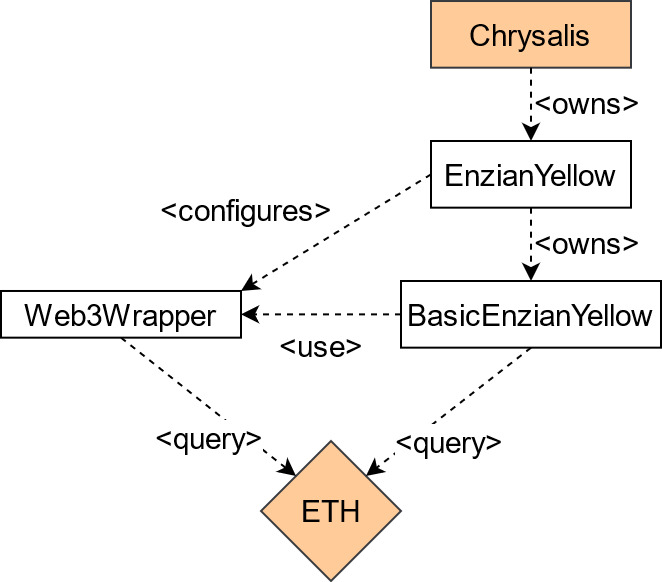
\includegraphics[height=0.5\textwidth]{gfx/enzian-original}
	\caption{Component structure of the original \emph{Enzian-Yellow} Repository. The components marked in orange are not part of Enzian-Yellow, but interact with it.}
	\label{fig:impr:enzian:original}
\end{figure}

As seen in figure \ref{fig:impr:enzian:original}, the architecture of \emph{Enzian-Yellow} consists of three parts, giving us the following understanding:
\begin{itemize}
    \item On the top, the name-giving class \emph{EnzianYellow} is the interface to the applications that use it (like \emph{Chrysalis}): It offers BPM-related methods like creating new processes or tasks and executing the latter, independent of the underlying Blockchain specifics. When constructed, it also instantiates \emph{BasicEnzianYellow} and \emph{Web3Wrapper}.
    \item \emph{BasicEnzianYellow}, as the name might suggest, is a specialization of \emph{EnzianYellow} (though not inheriting from it), offering the same kind of method signature as it's 'parent', but translating these BPM actions into the corresponding Blockchain-transactions. To make these transactions, it sometimes calls the \emph{Web3Wrapper} and sometimes directly queries the \emph{Web3} instance within.
    \item \emph{Web3Wrapper} wraps, as the name indicates, an instance of the class \emph{Web3}, which is the API used to connect and interact with a local \emph{Ethereum} node. It offers functions like deploying contracts, however doesn't fully implement all BPM functionality that \emph{EnzianYellow} offers.
\end{itemize}

\textbf{Tasks} \\[0.2em]
From the given structure, as well as some other observations, the following issues were selected to be solved in this restructuring:
\begin{itemize}
\nopagebreak
    \item The \textbf{Dependencies} in the code do not follow a strict hierarchy in the sense of a layer-based architecture, with each layer offering abstraction to and fully satisfying the functional demands of the layer above (Section \ref{sec:impr:enzian:dep}).
    \item In many places, multiple methods with different parameters have the same effect, allowing for \textbf{code duplicates}. Additionally, \textbf{construction} does sometimes not imply object initialization, leaving room for hard-to-explain errors and 'zombie states' (Section \ref{sec:impr:enzian:sig}).
    \item It is not immediately clear, where an \textbf{Expansion}, like adding another Blockchain protocol, would be tied into (Section \ref{sec:impr:enzian:exp}). 
    \item The overall \textbf{Transparency}, especially via log outputs, should be improved (Section \ref{sec:impr:enzian:log}).
\end{itemize}

\subsection{Improving the Dependency Hierarchy}
\label{sec:impr:enzian:dep}

\begin{figure}[h]
	\centering
	\captionsetup{justification=centering,margin=2cm}
	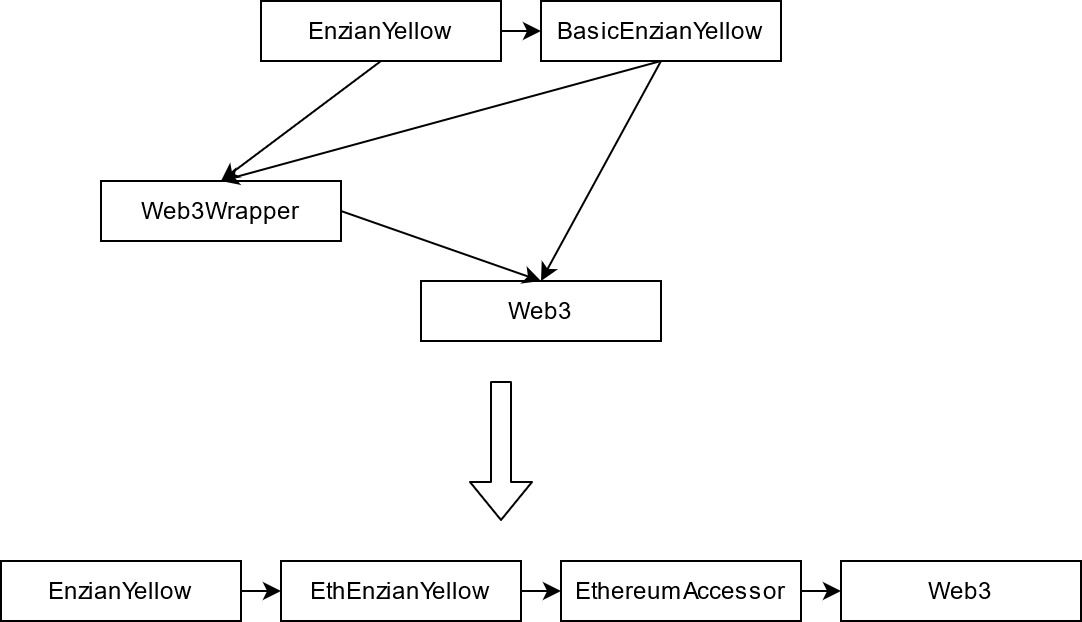
\includegraphics[height=0.5\textwidth]{gfx/enzian-dependencies}
	\caption{The dependency structure of the \emph{Enzian-Yellow} module before and after being reworked, sketched.}
	\label{fig:impr:enzian:dependencies}
\end{figure}

In a fully layered architecture, as we meant to achieve, one layer should never interact with another layer except that above and below. In \emph{Enzian-Yellow} that was not entirely the case. For example, the \emph{Web3Wrapper} object would do interactions with the Blockchain using the contained \emph{Web3} interface, yet the 'parent' object, \emph{BasicEnzianYellow}, would also directly access \emph{Web3}, essentially skipping the wrapper entirely. While this pattern is functional, it is hard to maintain when changes are made to a component, as abstractions of layers are not strict and changes therefore may affect more layers. To achieve a more strict layer-architecture, the following was done:
\begin{itemize}
    \item To fulfill every component's requirements towards lower layers, the first layer underneath was extended to offer all necessary methods, removing the need for layer-skipping.
    \item Code was moved to the specific place where it was meant to be, e.g. actions that required using \emph{Web3} would only be allowed inside the \emph{Web3Wrapper}.
    \item With delegations for every possible method in place, the dependency structure could now be flattened, as shown in figure \ref{fig:impr:enzian:dependencies}.
    \item Finally, in the new structure, a few components were renamed to better reflect their functionality - especially with future expansions in mind. \emph{BasicEnzianYellow} became \emph{EthereumEnzianYellow} and the \emph{Web3Wrapper} became the \emph{EthereumAccessor}.
\end{itemize}

\subsection{Method and Object Signatures}
\label{sec:impr:enzian:sig}

In the prototype system, code was significantly scattered and duplicated, offering the same functionality multiple times with differing parameters, like the example shown in figure \ref{fig:impr:enzian:sig-pre}. As this affects maintainability negatively, we sought to eliminate such redundancies wherever possible.

\begin{figure}[h]
	\centering
	\captionsetup{justification=centering,margin=2cm}
	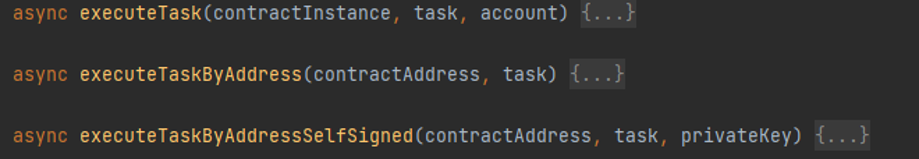
\includegraphics[width=\textwidth]{gfx/enzian-signatures-pre}
	\caption{The 'execute task' method signatures in the original system.}
	\label{fig:impr:enzian:sig-pre}
\end{figure}

Reducing the code scatter boiled down to finding the minimum information with which a method could be executed. In our example case, the \emph{contract instance} argument could be created from the \emph{contract address} - in fact, the instance was always internally created from the address. Additionally, for abstraction purposes, it should not be necessary for the above layers to use such contract instances. Similarly, The \emph{account} and \emph{private key} arguments are equivalent; we opted for only using private keys, as it is a string and therefore more compatible with higher layers, as well.

\begin{figure}[h]
	\centering
	\captionsetup{justification=centering,margin=2cm}
	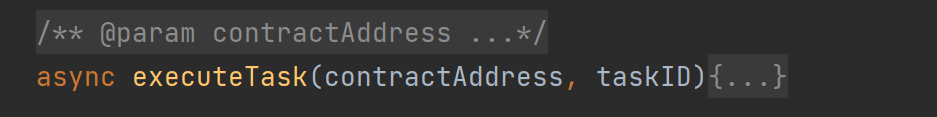
\includegraphics[width=0.7\textwidth]{gfx/enzian-signatures-post}
	\caption{The method signature from figure \ref{fig:impr:enzian:sig-pre} after being merged.}
	\label{fig:impr:enzian:sig-post}
\end{figure}

Additionally, some objects like \emph{Web3Wrapper} would allow being instantiated and configured without being initialized - like connecting to the Blockchain's endpoint, for example. It is generally recommendable to initialize an object immediately when instantiating it, as it could be created successfully while in an invalid state otherwise, leading to potentially hard to understand errors.

With the described changes, the previous example was reduced to the method signature shown in figure \ref{fig:impr:enzian:sig-post}, being a clear improvement, as was done in many other places in the code.

\subsection{Interface for Expansions}
\label{sec:impr:enzian:exp}

With the codebase cleaned up with the methods and principles described in the previous sections, it makes sense to tackle the next design question: How and where should an expansion to the existing system implemented?

\begin{figure}[h]
	\centering
	\captionsetup{justification=centering,margin=2cm}
	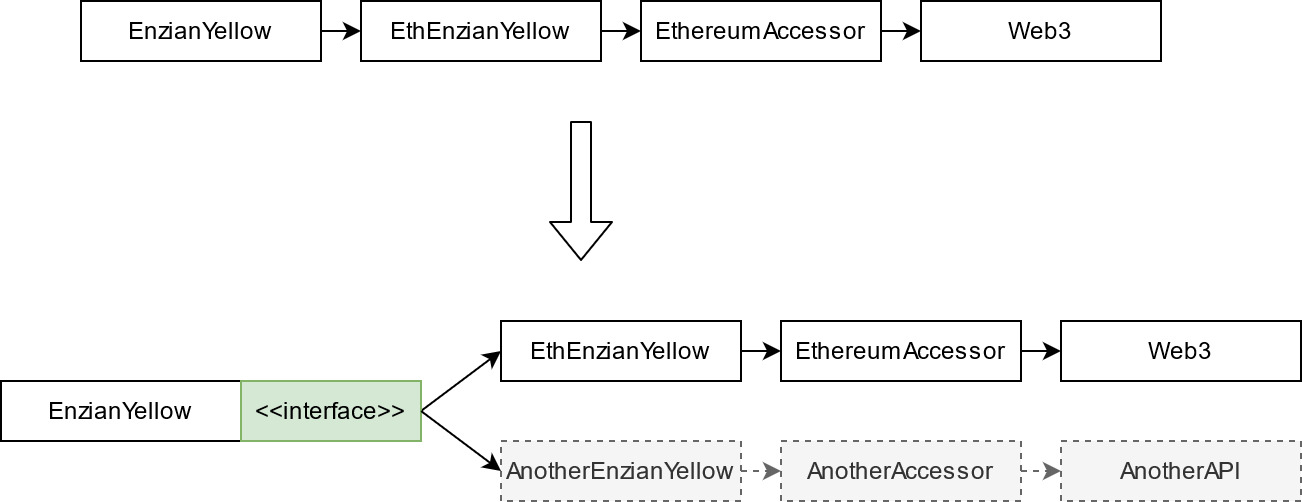
\includegraphics[width=\textwidth]{gfx/enzian-expansion}
	\caption{\emph{Enzian-Yellow}'s Structure before and after introducing an interface for expansion, with a sample expansion sketched in (grey).}
	\label{fig:impr:enzian:expansion}
\end{figure}

As the introduced naming scheme might have already hinted, the perfect way to put an expansion into the current system would be to offer replacements for \emph{EthereumEnzianYellow} that can fill it's signatures. In figure \ref{fig:impr:enzian:expansion} we sketched this as a proper interface, but note that JavaScript as a language does not support such constructs and is weakly typed, meaning that any object with the same method names and signatures may already replace \emph{EthereumEnzianYellow}, no inheritance or implementations needed.

Expanding the \emph{EnzianYellow} module with a new Blockchain of type 'x' is therefore quite simple: One must only make their 'xEnzianYellow' known to the parent class, \emph{EnzianYellow}, and define under which circumstances this new Blockchain application may be used. We opted for a simple constant, passed down to \emph{EnzianYellow} as a string to configure it. If "ethereum" (or, in fact, nothing) is passed for example, \emph{EthereumEnzianYellow} will be selected.

\subsection{Transparency}
\label{sec:impr:enzian:log}
To improve the application's transparency to the developer and partly the user, we've implemented a new logging strategy and added doc-strings throughout the code.

\begin{figure}[h]
	\centering
	\captionsetup{justification=centering,margin=2cm}
	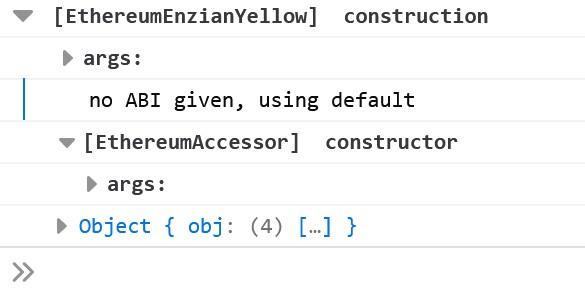
\includegraphics[width=0.5\textwidth]{gfx/enzian-transparency}
	\caption{An example of nested logging during construction of Enzian-Yellow.}
	\label{fig:impr:enzian:transparency}
\end{figure}

\textbf{Nested Logging} \\[0.2em]
A special functionality in JavaScript is log grouping, which is achieved by calling \texttt{console.group()} to open a group and \texttt{console.groupEnd()} to close it. Everything between these delimiters will be indented in the log, with most browsers also allowing to collapse a log group. We applied these calls at the beginning and end of many methods, including a call that prints all arguments the method received, creating a nested log structure like the one visible in figure \ref{fig:impr:enzian:transparency}. This allows the developer - and the user as well - to easily follow the call structure and the way arguments have been passed down, providing aid during debugging, for example. 

\textbf{Code Documentation} \\[0.2em]
Throughout the code, we also added doc-strings to most methods. This provides the developer with useful type hints as well as short descriptions of methods, where the name alone can not convey the full syntax and semantics. 

\subsection{Result}
\label{sec:impr:enzian:result}

As per the definitions of this task, the behaviour of the codebase has essentially not changed after implementing these improvements. However, the goals of maintainability and expandability were definitely reached, with unnecessary code scatter removed, transparency increased in many places and many structures simplified. \newline
The only opportunity missed is to separate \emph{Enzian-Yellow} into it's own secluded REST server, as this would've prevented the issue described in section \ref{sec:issues:integration}.
% !TEX root = ../chrysalis-report.tex
%
\section{Persistence layer}
\label{sec:impr:persistence}

In this section we will discuss the implementation of the Persistence layer of CHRYSALIS. We will list the problems solved by this tasks, details of the implementation both on the front- and backend side and results achieved by it. 

\subsection{Problem statement}
\label{sec:impr:persistence:problem}

Initially, when we got our hands on the project, CHRYSALIS stored all of the off-chain configuration data in the browser's local storage. Not only is it a safety concern (since the frontend user can easily manipulate data how they want), but also it is not reliable, since the browser's local storage could be cleaned on the user side and all of the data would be lost. 

The other point of concern was that the only way to access deployed process models was by explicitly typing in its contract address, which renders the user interface completely useless and ruins user experience. Furthermore, to pick a task for execution, one had to explicitly specify the id assigned to it after the parsing into enzian model, which the user might not have even noticed. Lastly, there was no constraints on the task identifiers that could be chosen, so the user was capable of choosing an incorrect one and getting an error. To combat that, we decided to implement a persistence layer, which would store all the off-chain information in a database, including information on associations between tasks and deployed processes. 

\begin{figure}[hbt]
	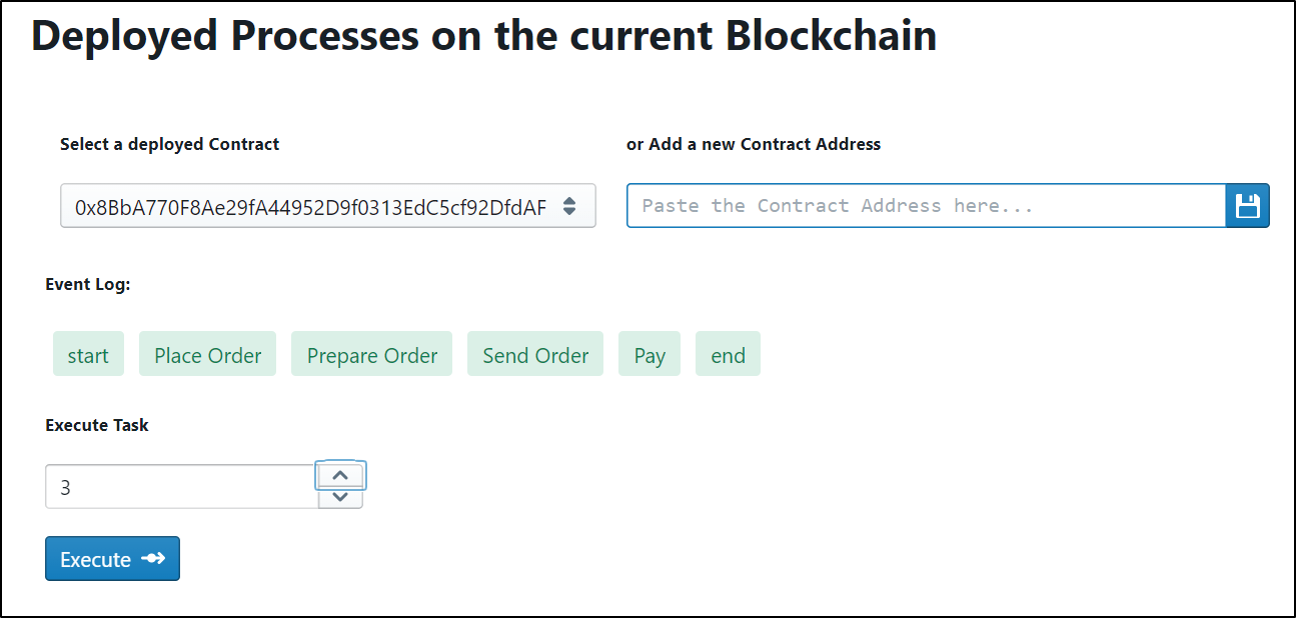
\includegraphics[width=\textwidth]{gfx/persistence_before}
	\caption{Process execution page before implementation of the persistence layer}
	\label{fig:impr:persistence:before}
\end{figure}

\subsection{Software stack}
\label{sec:impr:persistence:stack}

To implement this functionality we decided to build a separate REST-server. For the server's implementation framework express.js was chosen, since the entire project is in javascript and express.js is meant for RESTful API implementation. PostgreSQL was chosen as a database management system, mainly because it is widely used and optimized for production, but free at the same time (unlike, for example, Oracle). It also provides a wide array of object-relational functionality, which could be useful further in CHRYSALIS development. For exchange between the server and the database Sequelize ORM is used.

\begin{figure}[hbt]
	\centering
	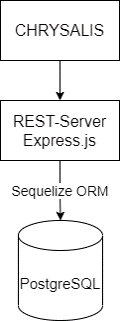
\includegraphics[width=.3\textwidth]{gfx/persistence_architecture}
	\caption{Persistence layer architecture}
	\label{fig:impr:persistence:architecture}
\end{figure}

\subsection{Backend}
\label{sec:impr:persistence:backend}

As it is required by Sequelize ORM and the express.js framework, the server code is divided into four packages: models, migrations, controllers and routes. Models contain a representation of database entities, including column datatypes, constraints, associations and cardinalities. Migrations contain scripts used for propagating the database schema created in the model package and all the changes made in that schema to the database. Every migration contains a function to propagate the changes and a function to undo them. The controller package contains the server's business-logic, the database interactions in particular. The routes package provides the REST-API endpoints to communicate with the server.
 
The database schema is rather simple and consists of six entities (apart from the system relations, which the Sequelize ORM needs to work). Those entities are: Process, task, connection, abi, setting and account. The entities "Process" and "Task" are self-explanatory. Connections contain information about blockchain networks that the user could connect to. Account contains information regarding user's account on the blockchain network, such as their private key for signing transactions. Abi is an entity containing compiled smart contract code for executing a process model and is deployed every time a new process is uploaded to the system. The "Settings" entity contains the current set of connection configurations, chosen by the user. Processes and Tasks are connected by a one-to-many association.

\begin{figure}[hbt]
	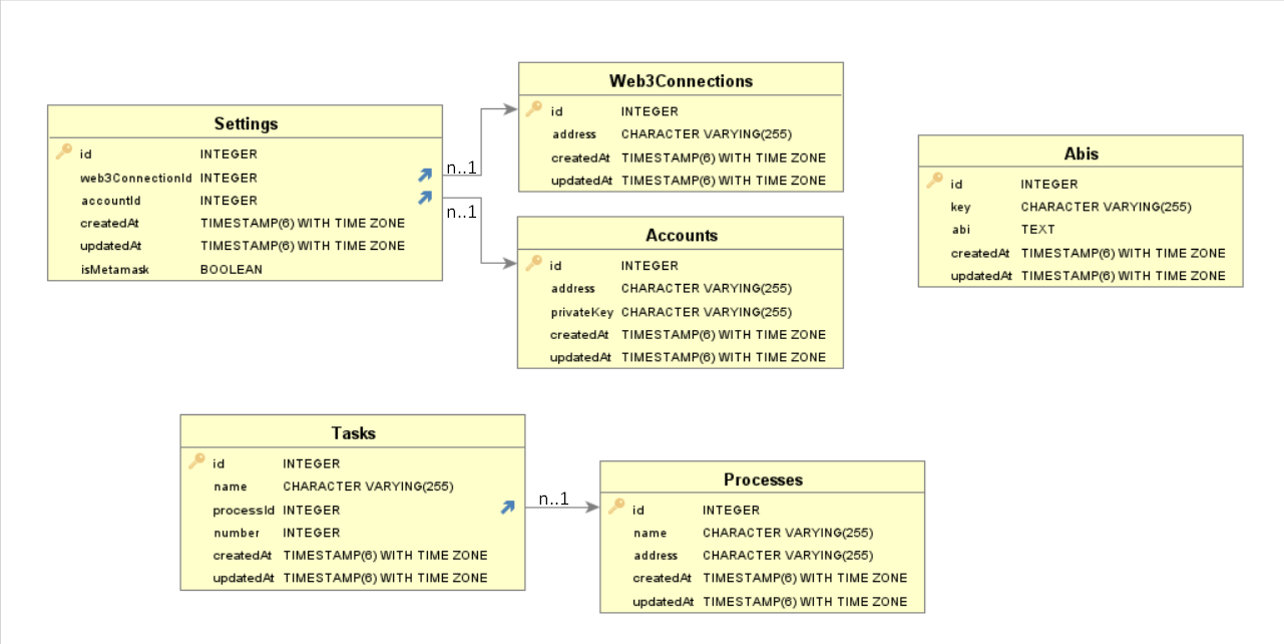
\includegraphics[width=\textwidth]{gfx/persistence_schema}
	\caption{Database schema}
	\label{fig:impr:persistence:schema}
\end{figure}

\subsection{Frontend}
\label{sec:impr:persistence:frontend}

On the frontend side we had to work within the confines of the existing application. The main means of RESTful exchange in react.js is Fetch-API. But the problem is that Fetch-API is very wordy and we would have to reuse large blocks lots of times, in every component of the application. Not only that, but one would have to call this API with a wide array of different parameters, depending on the caller's intention. So it was decided to implement some universal exchange handling functionality within the frontend application.

To implement this it was decided to create an ExchangeHandler class which is called by the application components to handle their requests. The components would pass it to the request method, URI and optionally data that they have to send, and then based on the method the exchange handler would find the appropriate instance of one of the sender classes and call them to execute the request. These sender classes are GetRequestSender, PostRequestSender, PatchRequestSender and DeleteRequestSender. They are instantiated and kept in the SenderRepository class. It contains a map with request methods as keys and sender instances as values. The exchange handler gets an appropriate sender from this map and calls its send() method to make a request to the server, returning a special promise objects, which provides methods to specify a logic, that should be executed once the response is received.


\begin{figure}[hbt]
	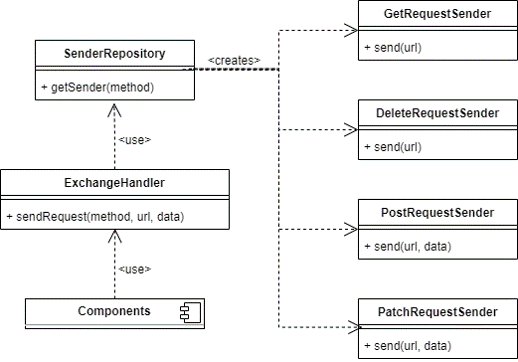
\includegraphics[width=\textwidth]{gfx/persistence_exchange}
	\caption{Database exhange module}
	\label{fig:impr:persistence:exchange}
\end{figure}

\subsection{Result}
\label{sec:impr:persistence:result}

After these changes, all of the off-chain data was moved from the local storage to a separate database, improving safety and reliability. User experience was also significantly improved, since it became possible to choose deployed processes by their name from a list provided by the server, as well as to choose from tasks associated with the process by their name as well. The functionality of retrieving deployed processes by their contract addresses (if they are not present in the database) was preserved as well, but it underwent slight changes to make it compatible with the new architecture, and these changes will be discussed in the smart contract optimization section.

\begin{figure}[hbt]
	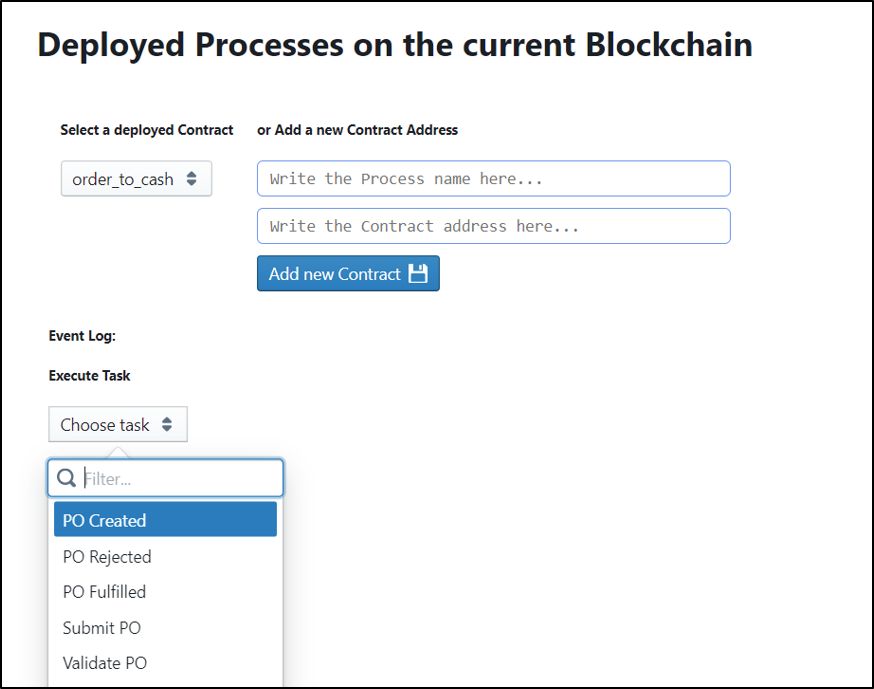
\includegraphics[width=\textwidth]{gfx/persistence_after}
	\caption{Process execution page after the improvements}
	\label{fig:impr:persistence:after}
\end{figure}



% !TEX root = ../thesis-example.tex
%
\section{Hyperledger-based Application}
\label{sec:impr:hl}



With the interfaces needed to expand the system being in place, we deemed it a good next step to add another Blockchain protocol. Specifically, we chose \emph{Hyperledger}. The application was expanded with all necessary components implemented and tested, although the front-end still has problems trying to pack this new addition and sending it to the user's browser. This issue is elaborated in section \ref{sec:issues:integration}. This chapter will focus on firstly giving a broad overview of Hyperledger in section \ref{sec:impr:hl:basics} and then following up with detailing the implemented expansion in the later sections. \newline
All information about Hyperledger and how it is used was sourced from the documentation version 2.2 at \cite{hyperledger}.

\subsection{Hyperledger as a Ledger Protocol}
\label{sec:impr:hl:basics}

To explain how the Systems of \emph{Hyperledger Fabric} work and what special features they offer, it makes sense to offer a comparison to the \emph{Ethereum} Blockchain - feature by feature. \emph{Hyperledger} wants to set itself apart by being a business-oriented information transfer protocol (hence, a shared ledger). Values, like tokens (e.g., \emph{Bitcoin, Ethereum}), are not a fundamental part of it.

\textbf{Authorization} \\[0.2em]
If configured, a Hyperledger Network will be split into groups, called organisations. Each organisation has a (potentially distinct) \emph{Certificate Authority (CA)}, through which membership in an organization is validated for every peer and account. Therefore, if one wants to interact with the network by for example invoking a smart contract, they must first be authenticated  by the CA. The CA even allows for group roles, so not every query to the network is accessible to everyone. These group roles were not further regarded in this task, however.

\textbf{Block Sealing} \\[0.2em]
I.e., the process of adding blocks to the Blockchain and therefore changing it's active state and log, is an essential part of Blockchain technology. In more known protocols like \emph{Bitcoin} or (at least at the time of writing) \emph{Ethereum}, the content of the next block is decided by the node that first managed to solve a cryptographic puzzle - the solving of this puzzle is called \emph{mining}. This, however, means that the time of sealing a block is somewhat random - and a bidding process is necessary to convince the block sealer of writing one's data. \newline
Hyperledger circumvents this competition-based method and instead introduces an \emph{orderer} node, which generally tries to apply block-additions in a first-in-first-out fashion (and accounts for concurrency issues). This means a more reliable way of querying the blockchain, since all actions are executed as fast as resources allow, and also because competing peers are treated equally instead of based on their bid. \newline
Additionally, from a security standpoint, such a network can not as easily be 'poisoned' (by holding such a large amount of tokens or mining power that the holder can essentially decide which transactions to incorporate), since the finances and mining capacities of peers are disregarded completely.

\begin{figure}[h]
	\centering
	\captionsetup{justification=centering,margin=2cm}
	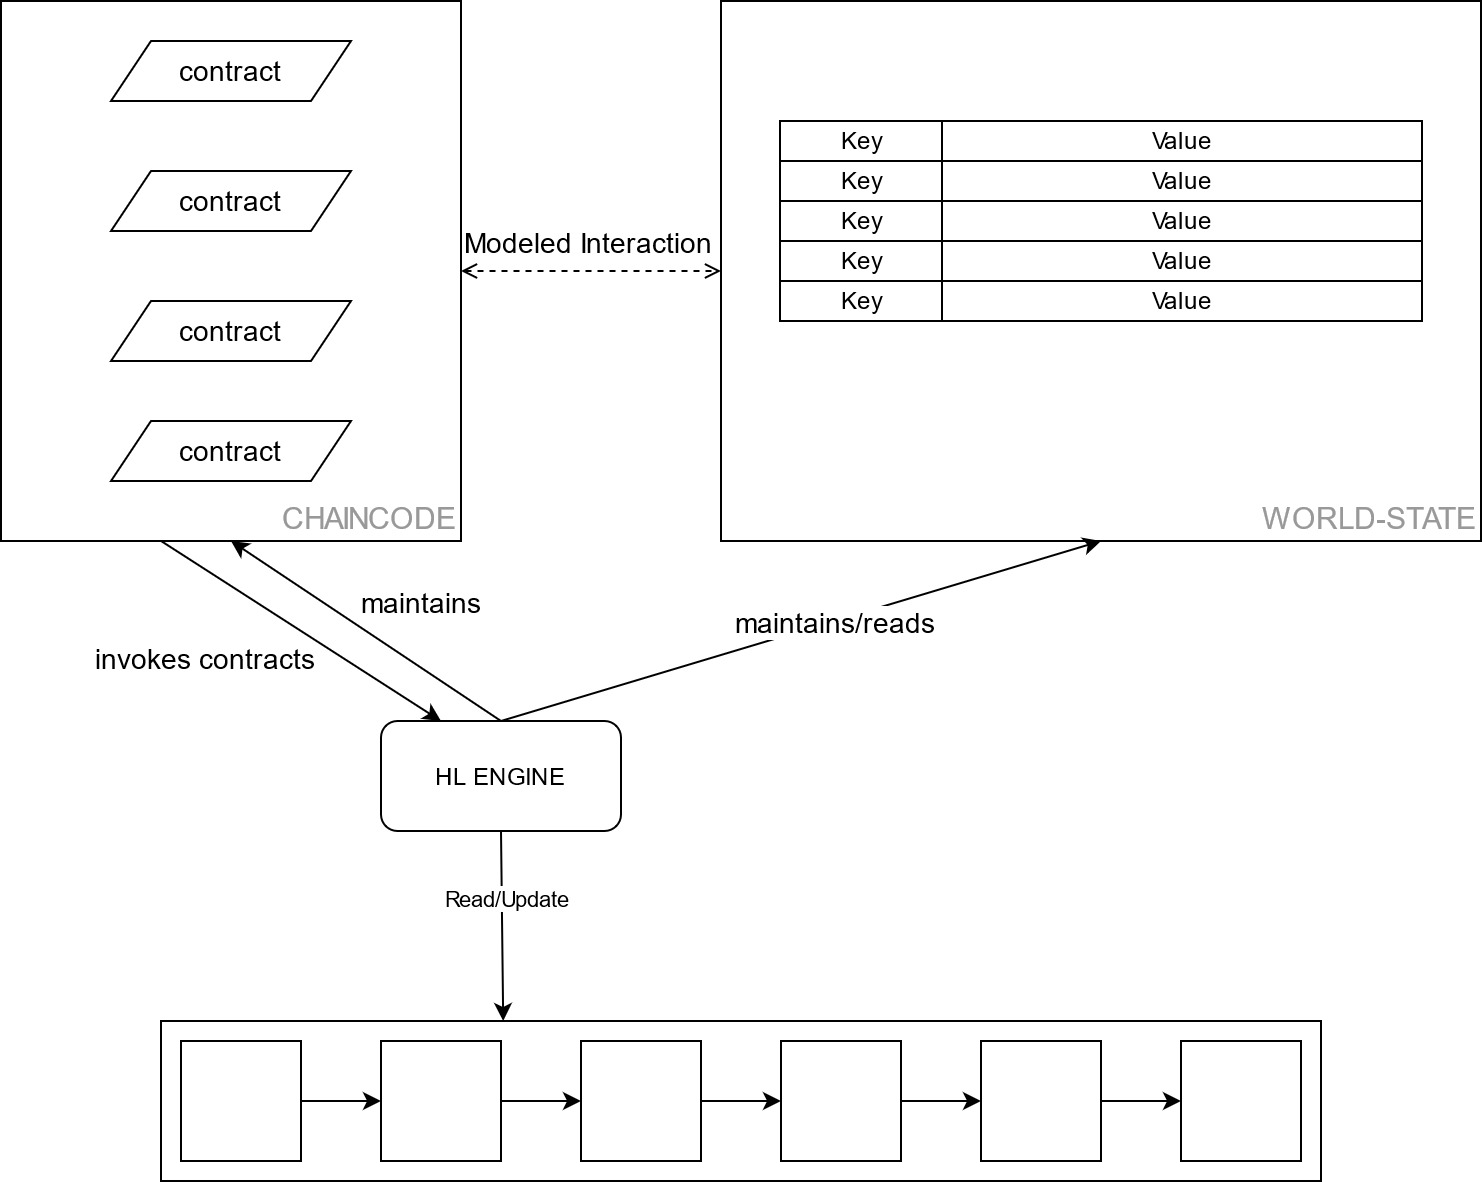
\includegraphics[height=0.7\textwidth]{gfx/hl-abstraction}
	\caption{Sketch of \emph{Hyperledger's} abstraction mechanism, \emph{HL} standing for \emph{Hyperledger} here.}
	\label{fig:impr:hl:basics:abstraction}
\end{figure}

\textbf{Abstraction: \emph{World State \& Chaincode}} \\[0.2em]
As depicted in figure \ref{fig:impr:hl:basics:abstraction} by an 'engine' component (although this is a big simplification), Hyperledger has functions in place to display the underlying Blockchain's contents in a more abstract way, so that the user or developer doesn't need to bother with physical addresses, but may instead find them in a more human-readable format. \newline
The \emph{World State} Container is a synchronous representation of all data present in Hyperledger's underlying Blockchain, meaning that the data points present are always a representation their most recent update. Additionally, the World State is arranged like a dictionary, so that every structure inside is reachable by a key, defined by the user itself. This way, the programmer doesn't have to worry about physical addresses of the data. \newline
In the \emph{Chaincode} container(s) one can find the Smart Contract objects one would also find in other Blockchain application. However, these contracts are not stateful and therefore do not contain any data besides the location of the World State, where the data may be contained. In comparison, an \emph{Ethereum}-based contract may have private data and would therefore be stateful. Additionally, Chaincodes are also invocable via name, specifically by a combination of the parent contract name and the function that is to be executed.

\subsection{Component Overview}
\label{sec:impr:hl:requirements}

\begin{figure}[h]
	\centering
	\captionsetup{justification=centering,margin=2cm}
	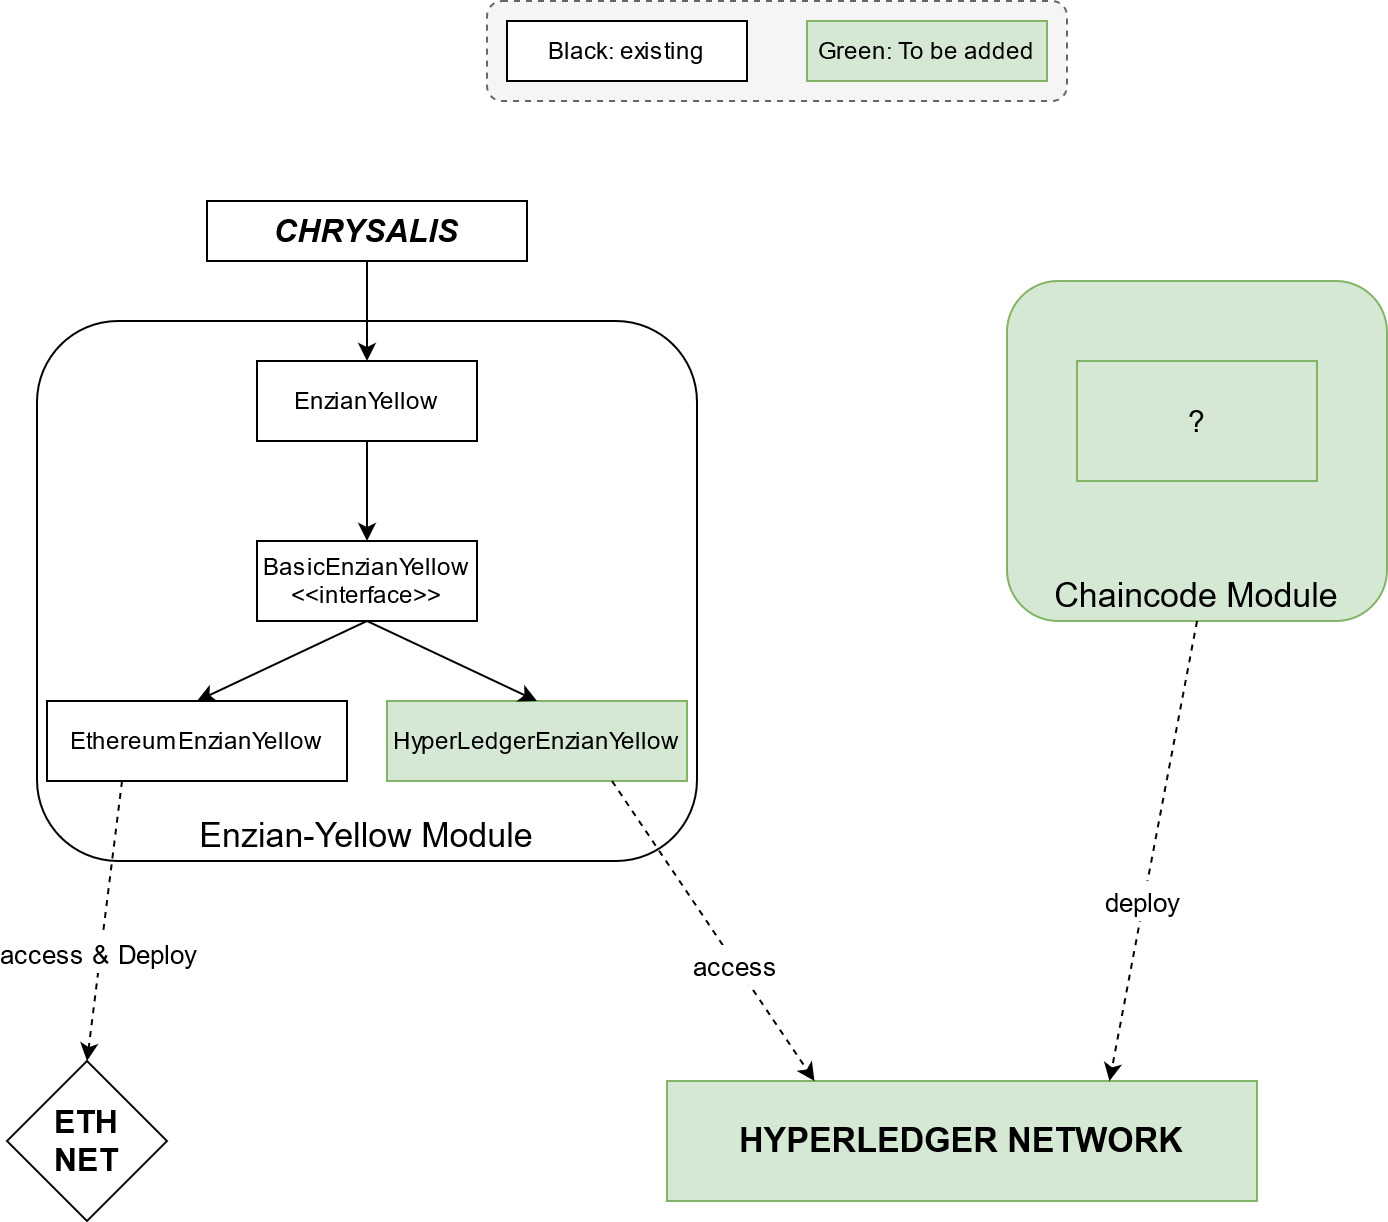
\includegraphics[width=\textwidth]{gfx/hl-structure}
	\caption{Planned and implemented module structure after adding the \emph{Hyperledger} protocol}
	\label{fig:impr:hl:structure}
\end{figure}

Three components are needed to build a running Hyperledger-based application for the Chrysalis project. \newline
First of all, a Hyperledger Network must be established, so that all necessary structures can be deployed there. Secondly, being the most complex component of the three, the Chaincode must be defined along with the data structures it uses. This module may be written and deployed in generic JavaScript thanks to Hyperledger's flexibility regarding the deployed language (e.g., this module could also be written in \emph{Go}). As per Hyperledger's requirements, the module must be contained in a separate package that can locally install dependencies and can be packed into a compressed file. Once this package is deployed, an API is needed in \emph{Enzian-Yellow} to access the network and use the deployed components. This step is fairly straightforward, since Hyperledger Fabric provides this API and the structure of the \emph{HyperledgerEnzianYellow} can mostly be mirrored from that of \emph{EthereumEnzianYellow}.

\subsection{Test-Network}
\label{sec:impr:hl:network}

To keep development effort low, the Hyperledger Network, where the contracts and data may be deployed, was not built from scratch, but instead the "test-network" from Hyperledger's \emph{fabric-samples} repository was used. This network came with the features stated below.

\textbf{Network Deployment:} Instead of having to configure every network node, having to start it manually and registering it to the network, the test-network spares the developer from this work by making a running network with isolated components available as a composition of \emph{Docker}-Images. Additionally, with the help of pre-written scripts, the user may easily instantiate that composition.

\textbf{Reset functionality:} With a pre-written script, the developer may also simply wipe the entire network and bring it down. This makes development easier, since no trace (potentially even illegal states) of previous work will be left on the Blockchain.

\textbf{Multi-Organization Scenario:} If instantiated with the right parameters, the network would come up with two organizations created, both containing one network peer each and reporting to a certificate authority. This configuration is useful, since the developer can make sure their application would run in a realistic scenario where their application and contracts must be validated by all network-registered organizations. The test-network also offers a lot of helpful scripts to make interactions with it a bit less cumbersome, e.g., so that Chaincodes may be deployed with less steps.

\subsection{Representation of Processes}
\label{sec:impr:hl:datastructure}

It makes sense to split the data model deployed onto the ledger into two parts: The first defines how a JavaScript object may be represented inside the \emph{World State} as well as in memory and how these two versions are to be synchronized. The second part, building on those definitions, defines how a process as well as it's tasks shall be modeled as such objects, how they interact and how they may be operated upon. The resulting components are visible in figure \ref{fig:impr:hl:data} and described below.

\textbf{Objects on the World State} \\[0.2em]
As the World State acts like a dictionary, any data placed on it is modeled as an extension of the class \emph{State}. This State object defines its own key with which it is found on the dictionary-like structure, as well as a static method to serialize and deserialize it to/from a JSON representation, as it has to be stored in a more permanent form. \newline
In addition to this data class, a 'manager' object is needed, in our case of the type \emph{StateList}, to store the location of the World State itself, to write or update deserialized State objects onto it, and to cast the 'rehydrated' objects back onto the correct class.

\begin{figure}[h]
	\centering
	\captionsetup{justification=centering,margin=2cm}
	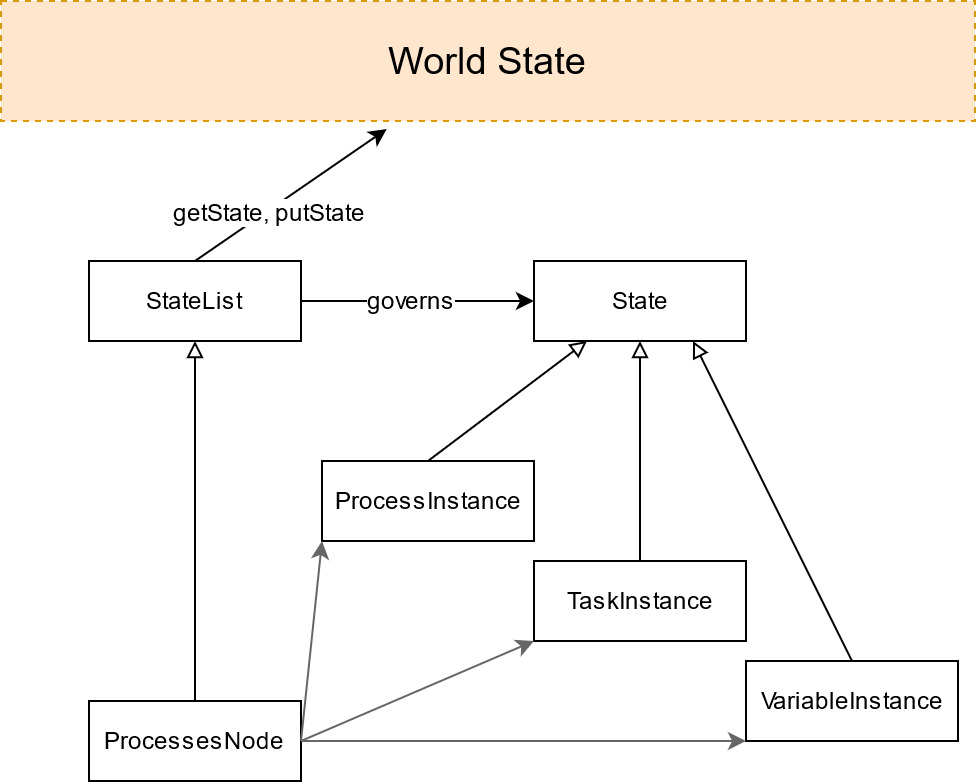
\includegraphics[width=0.8\textwidth]{gfx/hl-data}
	\caption{Data Structure deployed on the World State (State) as well as the objects that actively read and write on it (StateList)}
	\label{fig:impr:hl:data}
\end{figure}

\textbf{Process Representation} \\[0.2em]
With the definitions of \emph{State} and \emph{StateList} given, we can now implement the process structure as a simple extension of those, mostly not having to worry about the internals of the World State. 
\begin{itemize}
    \item \textbf{ProcessInstance}, being an extension of State, is the structure that binds an active process together: It stores the keys that point toward its subordinated Tasks and Variables, and also contains the event log, which is an ordered list of task IDs, appearing in the order the tasks were executed (a newly created ProcessInstance would therefore contain an empty log). As the ProcessInstance is the 'root' object of the data structure, it's Key is simply defined as a positive integer.
    \item \textbf{TaskInstance}, representing the Task State, contains - besides it's key and ID - all necessary data that makes up tasks in BPMN: A name, a list of competing tasks and completed task IDs required for execution, and so on. Additionally, to model BPM gateways it contains a \emph{precedingMergingGateway} attribute as well as a \emph{decision} structure, similar to the structures defined in the Ethereum application. The key is defined as follows: \emph{[key of parent process]:task:[task ID]}, e.g., \texttt{0:task:0} for the first task of the process 0.
    \item \textbf{VariableInstance}, lastly, is a simple wrapper for a value of a given type, with a log of previous values as an addition. Currently, only variables of type integer and string are supported. The key is defined as follows: \emph{[key of parent process]:var:[variable ID]} - also showing why the middle section differentiating between tasks and variables is needed: Variable and task IDs may clash and must therefore be expanded by some prefix.
\end{itemize}
The \textbf{ProcessesNode} class, extending StateList, acts as a gateway to the previously defined objects, offering the usual \emph{get, set} and \emph{update} methods. Also, since it makes sense to immediately write every action on the data structure onto the World State after executing it to prevent bugs, ProcessesNode also offers many BPM-based functions like \emph{executeTask}, therefore encapsulating a lot of Process logic as well. Objects of this class are meant to make it possible to interact with the process model entirely without knowing the underlying model, only using the provided keys. \newline
How this ProcessesNode finds its way into a Chaincode, however, will be explained in the next chapter.

\subsection{Process Deployment and Execution}
\label{sec:impr:hl:chaincode}

A Smart Contract (Chaincode) in Hyperledger Fabric, as well as the data structure, can be written in multiple supported programming languages, including JavaScript, which was used here. Implementing it is as simple as creating a class that extends the \emph{Contract} class from the Fabric API, as seen in figure \ref{fig:impr:hl:contract}.

\begin{figure}[h]
	\centering
	\captionsetup{justification=centering,margin=2cm}
	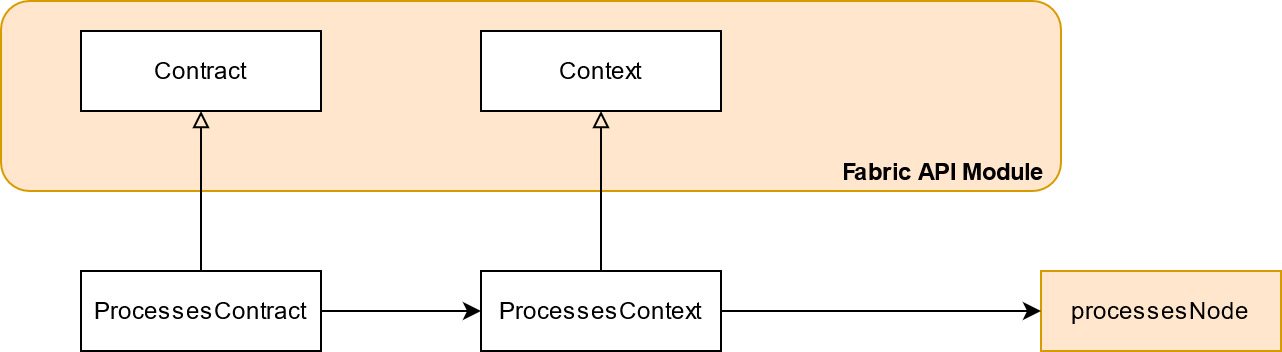
\includegraphics[width=\textwidth]{gfx/hl-contract}
	\caption{Structure of a Chaincode (Contract) together with it's gateway object that points to the World State (Context)}
	\label{fig:impr:hl:contract}
\end{figure}

\textbf{Contracts} \\[0.2em]
Defining what would be an invocable contract from the outside is as simple as extending the \emph{Contract} class and giving the extension a method: Users will be able to invoke this function by its name coupled with the class's name, e.g., "ProcessesContract" and "createProcess", together with it's arguments. However, a few special rules apply here: Firstly, while parameters and return values can be generic JavaScript objects that do not have to be serialized, all non-primitive arguments must be transferred via \emph{Buffer} to account for the networking between the caller and the callee. Secondly, the contract methods will always be provided a \emph{Context} object (see next passage for details) as first positional argument. This context will be handed to the method by the Hyperledger API, not the caller, therefore only the second argument and all those after may be used for argument passing.

\textbf{Context} \\[0.2em]
The Context, as described before, is another object provided by Hyperledger's API and handed to every smart contract during execution. Foremost, it contains the network-\emph{stub}, which is the gateway to the World State. We can now extend this Context into \emph{ProcessesContext}, that always contains a newly instantiated ProcessesNode object, therefore also giving access to all the data structures and logic as we defined them in section \ref{sec:impr:hl:datastructure}. During instantiating, the ProcessesNode is also handed a reference to the stub, so that it may have an access point to the World State. To make it clear to Hyperledger's API that our Chaincode is supposed to use this version of Context, we override the Chaincode's method \emph{createContext} to return our version instead of the default one. 

With these two components, it is now clear how a contract invocation results in manipulations or queries on the processes: When a method of ProcessesContract is invoked, it is handed the ProcessesContext and uses it to access ProcessesNode to then execute all process-related logic there. The whole interaction is currently purely based on passing and returning keys and primitive construction parameters, however it would also be possible for the caller to receive objects from the data structure as copies of their current state - still, it should generally be disallowed to write self-made objects to the network, as this might cause trust issues.

\subsection{Integration into Chrysalis}
\label{sec:impr:hl:integration}

From the side of HyperledgerEnzianYellow, interaction is fairly simple. Due to the underlying interaction model in the Hyperledger network being similar to the model deployed to the \emph{Ethereum} network, the general structure of HyperledgerEnzianYellow is basically the same as that of EthereumEnzianYellow. \newline
When HyperledgerEnzianYellow is instantiated, the HyperledgerAccessor is also constructed, building up a working connection to the Hyperledger network during construction (or throwing, if the connection fails). Currently, provided arguments aren't used, but instead read from a static definition, as an integration error (see section \ref{sec:issues:integration}) made using it properly impossible. \newline
Once the connection is built, the accessor can then freely pull a Chaincode by simply specifying the correct name, being returned an interface object. This interface can then be used to invoke the contracts by name and handing over parameters, as if the method was local. Using the previously defined Chaincode, HyperledgerEnzianYellow can offer the same functionality for BPM as EthereumEnzianYellow with the same parameters. The only difference is that the process addresses are in fact structured keys instead of proper addresses.

\subsection{Result}
\label{sec:impr:hl:result}

All in all, the task of implementing a Hyperledger-based process execution engine as a prototype can be considered successful and fruitful. The Hyperledger Smart Contracts are able to mirror the Ethereum Contracts, can be deployed on a running system successfully and can be connected to - especially by HyperledgerEnzianYellow. From a BPM perspective, the Hyperledger application fulfills all required functions and even partly surpasses Ethereum in a few features:
\begin{itemize}
    \item \textbf{Execution Speed:} As Hyperledger doesn't rely on mining to sign and validate new additions to the Blockchain, the deployed contracts can be invoked with fairly low delay - about two seconds per invocation. A direct comparability with Ethereum is not given, though: A mining-based protocol can technically be sped up massively by adding more miners and reducing the hashing difficulty of the mining puzzles. Still, Hyperledger's test-network is rather feature-rich and probably contains a lot of overhead that might not be needed in our case, and might also be a lot quicker if optimized.
    \item \textbf{Reliability:} Compared to mining blocks, adding them after a consensus is not based on random numbers. Therefore, the time between a contract invocation and the completion of the underlying transaction is extremely constant. In Ethereum's case, we saw huge discrepancies between the times individual transmissions took.
    \item \textbf{Readability:} As a small bonus, all addresses Hyperledger uses - even internally - are developer-defined and therefore have a human-readable structure, like those of the process data structure defined in section \ref{sec:impr:hl:datastructure}, and therefore make development and back-end work easier and more transparent even without usage of a persistence layer.
    \item \textbf{Efficiency:} Without mining, we perceived a significant reduction in processing load on the Hyperledger application compared to the Ethereum version. For example, where the Hyperledger application occupied a few threads with barely any load on the processor, the Ethereum miner alone (before process Chrysalis even ran), needed to put multiple processor cores on full load only to facilitate a transaction delay low enough to comfortably work with. This issue might not arise on more powerful server architectures, though.
\end{itemize}
% !TEX root = ../chrysalis-report.tex
%
\section{Ethereum overhaul}
\label{sec:impr:eth}

In this section we will discuss improvements regarding the smart contract structure of the project. Smart contracts are used for the deployment and execution of process instances within the system. They contain structures and methods for creation and handling of tasks and control flow decisions. For each process instance one new instance of the BasicEnzian smart contract is deployed.

\subsection{Problem statement}
\label{sec:impr:eth:problem}

In its initial state, the project kept all of its on-chain functionality in one single smart contract. There was no separation of concerns, a lot of the universal, non instance-specific functionality was left in, which lead to not only poor scalability and reusability of the smart contract code in the future, but also to significant performance costs, which, on the ethereum network, are measured in a unit called "gas". Gas consumption defines how much computational power the network needs to execute a certain operation, which then determines how much currency should be transferred from the account of a node requesting to execute this operation, to the account of the owner of the node executing it. So, in case of Ethereum, performance costs literally translate to money spent, that is why the main goal of the optimization was to minimize them. The listing below provides an example of code redundancy within the smart contract functionality. It contains a part of the task execution function, and as can be seen, mostly consists of parts which do not have to be in the contract, since they are independent from any specific process instance, and could be delegated to external components.

\lstinputlisting[style=java,caption=Task execution before the optimization]{progs/executeTask-before.txt} 

\subsection{Solution}
\label{sec:impr:eth:solution}

To achieve this, we had to optimize the most expensive operation in our system: smart contract deployment, since it happens for every new process instance in the system. Also the issue of reusability of components becomes more crucial because as the project will become progressively more complex in the future, the on-chain functionality will do so as well. So, we have to split the smart contract code into elementary parts, which would allow to implement new features by adding and deploying new modules, using existing ones, instead of rewriting and redeploying everything, which would also decrease performance costs during future development.

As an implementation model for this task clean architecture was chosen, since this model is designed to increase reusability of application components and overall scalability of the application. The main principle of this model is that all the modules are divided into three layers: domain layer, application layer and presentation layer. Domain layer defines structures and entities used in the application and basic objects carrying its state. The application layer, or middle layer, contains business logic of the application, the modules responsible for its behaviour and dealing with the object from the domain layer. The presentation layer provides entry points for external systems and users, that call functions and methods of the middle layer. The main requirement is that modules can only interact either with the modules from the same layer or the inner layer modules.

\subsection{Implementation}
\label{sec:impr:eth:implementation}

On the domain model layer, the libraries containing structs defining the objects of a process model along with the process state were implemented. These libraries were TaskEntities, DecisionEntities and ProcessEntities.\newline
The TaskEntities library defines the structure of a process task, which contains information on Task's name and id within the process instance, its completion state, as well as the set of requirements, that have to be fulfilled for this task to be up for execution. It also contains a reference to a Decision object, which is described in the DecisionEntities library.\newline
The DecisionEntities library defines structures and enumerators needed for evaluating control flow requirements in the gateways of a process model. The decision structure itself contains information on the gateway type, variables compared as well as the comparison operator for those variables. The enumerators containing gateway types and operators are also defined in this library.\newline
The processEntities library defines the structure containing information on the process structure and state. It contains the process' tasks, its integer variables and string variables.\newline
On the application layer there are two libraries: TaskLibrary and DecisionLibrary. TaskLibrary implements methods to create tasks on the process initialization, as well as methods to handle execution of tasks including evaluation of task requirements. To evaluate gateway conditions it calls the DecisionLibrary, which implements appropriate functionality.\newline
The presentation layer consists of the BasicEnzian smart contract, which provides entry points for the EnzianYellow library to interact with, as well as keeps the state of the process instance and its event log. 

\begin{figure}[h]
	\centering
	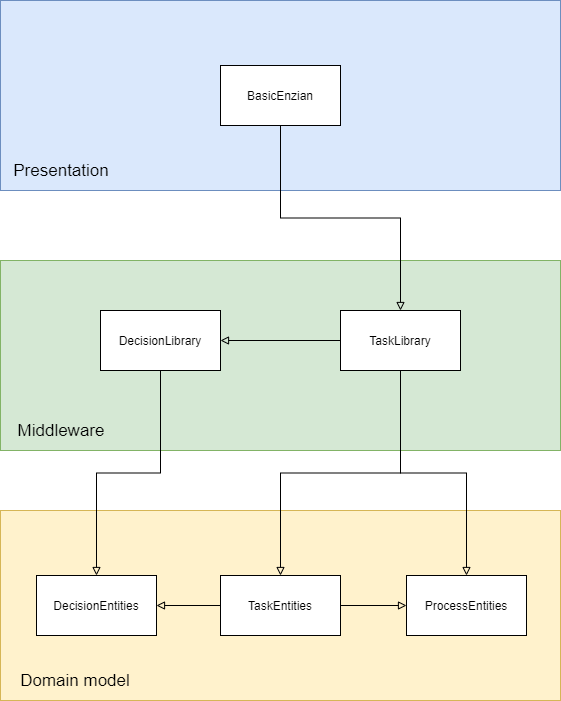
\includegraphics[width=0.5\textwidth]{gfx/eth-contracts}
	\caption{Structure of the ethereum smart contracts}
	\label{fig:impr:eth:contracts}
\end{figure}

\pagebreak

\subsection{Result}
\label{sec:impr:eth:result}

As an outcome of the smart contract overhaul, the structure of the smart contract code became more scalable and flexible, and it was divided into small modules which can be reused in the new contracts developed further down the line.
Other than that, the cost of process instance deployment was lowered from ~4300000 gas to ~3600000 gas, and overall the code became much cleaner, which could be seen in the following listing, which showcases the same function handling task execution. After the refactoring most of the method's logic is incapsulated in the TaskLibrary, which is called, and then the results from the library function are used to update the process state.



\lstinputlisting[style=java,caption=Task execution after the optimization]{progs/executeTask-after.txt} 


	
% !TEX root = ../thesis-example.tex
%
\chapter{Concepts}
\label{sec:concepts}

\cleanchapterquote{Users do not care about what is inside the box, as long as the box does what they need done.}{Jef Raskin}{about Human Computer Interfaces}

\Blindtext[2][1]

\section{Concepts Section 1}
\label{sec:concepts:sec1}

\Blindtext[2][2]

\section{Concepts Section 2}
\label{sec:concepts:sec2}

\Blindtext[3][2]

\section{Concepts Section 3}
\label{sec:concepts:sec3}

\Blindtext[4][2]

\section{Conclusion}
\label{sec:concepts:conclusion}

\Blindtext[2][1]
 
% !TEX root = ../thesis-example.tex
%
\chapter{Concepts}
\label{sec:concepts}

\cleanchapterquote{Users do not care about what is inside the box, as long as the box does what they need done.}{Jef Raskin}{about Human Computer Interfaces}

\Blindtext[2][1]

\section{Concepts Section 1}
\label{sec:concepts:sec1}

\Blindtext[2][2]

\section{Concepts Section 2}
\label{sec:concepts:sec2}

\Blindtext[3][2]

\section{Concepts Section 3}
\label{sec:concepts:sec3}

\Blindtext[4][2]

\section{Conclusion}
\label{sec:concepts:conclusion}

\Blindtext[2][1]
 
% !TEX root = ../chrysalis-report.tex
%
\chapter{Conclusion}
\label{sec:conclusion}

\section{Overview of the work}
\label{sec:conclusion:overview}
Over the course of this project we have overhauled the CHRYSALIS application structure on all levels of the architecture. First, significant changes were made to the overall codebase of both the business-logic library and the web application. The project codebase became cleaner and ready for future changes and additions. These changes have ensured simpler and more efficient development in the future.

Other than that, the persistence layer was introduced, providing safer and more reliable storage for the off-chain data and, by extension, laying the  foundation for the better user experience overall. On top of that the project's smart contracts have undergone a complete restructuring. This has lowered the performance costs of the on-chain operations as well as also prepared the project for the addition of new functional elements. Finally, we have implemented integration with the hyperledger network, thus making the system more flexible and adaptable to different environments.

The analysis of Caterpillar and its comparison with CHRYSALIS has shown that even though CHRYSALIS project, compared to Caterpillar, is still in its infancy, it already has leverage over the older and longer developed system in terms of user experience and in some cases even in performance costs, which shows its great potential.

In its current stage, the project offers a simple platform for decentralized interorganizational process management, it enables deployment end execution of simple process models utilizing a blockchain network, though it is limited in scope, especially in terms of support of more advanced BPMN features, which could be improved during further development of the project

\section{Future development}
\label{sec:conclusion:future}

From a purely technical standpoint, the web application needs migration to the newer version of Webpack, to enable support of some libraries incompatible with the older versions, especially the ones related to Hyperledger integration. 

There are still a lot of improvements, that could be made to CHRYSALIS until it reaches production, for example, support of such BPMN features as service tasks or script tasks, using smart contracts as services or scripts, or support for other process modelling notations. In the persistence layer, there has also been laid the groundwork for the future inclusion of user system with the connection settings being configurable for every individual user. Introduction of the user system would allow to implement role-binding policies for actors participating in the process, which is crucial for interorganizational process modelling.  Implementation of a process modelling tool could be another point of improvement to not force the users to create and run their process models using separate applications. 
\cleardoublepage

% --------------------------
% Back matter
% --------------------------
{%
\setstretch{1.1}
\renewcommand{\bibfont}{\normalfont\small}
\setlength{\biblabelsep}{0pt}
\setlength{\bibitemsep}{0.5\baselineskip plus 0.5\baselineskip}
\printbibliography[nottype=online]
\printbibliography[heading=subbibliography,title={Websites},type=online,prefixnumbers={@}]
}
\cleardoublepage

\listoffigures
\cleardoublepage

\listoftables
\cleardoublepage

% !TEX root = ../thesis-example.tex
%
%************************************************
% Declaration
%************************************************
\pdfbookmark[0]{Declaration}{Declaration}
\chapter*{Declaration}
\label{sec:declaration}
\thispagestyle{empty}

You can put your declaration here, to declare that you have completed your work solely and only with the help of the references you mentioned.

\bigskip

\noindent\textit{\thesisUniversityCity, \thesisDate}

\smallskip

\begin{flushright}
	\begin{minipage}{5cm}
		\rule{\textwidth}{1pt}
		\centering\thesisName
	\end{minipage}
\end{flushright}

%*****************************************
%*****************************************

\clearpage
\newpage
\mbox{}

% **************************************************
% End of Document CONTENT
% **************************************************
\end{document}
